\documentclass[journal,12pt,twocolumn]{IEEEtran}

\usepackage{setspace}
\usepackage{gensymb}
\singlespacing
\usepackage[cmex10]{amsmath}

\usepackage{amsthm}

\usepackage{mathrsfs}
\usepackage{txfonts}
\usepackage{stfloats}
\usepackage{bm}
\usepackage{cite}
\usepackage{cases}
\usepackage{subfig}

\usepackage{longtable}
\usepackage{multirow}
\usepackage{enumitem}
\usepackage{mathtools}
\usepackage{steinmetz}
\usepackage{tikz}
\usepackage{circuitikz}
\usepackage{verbatim}
\usepackage{tfrupee}
\usepackage[breaklinks=true]{hyperref}
\usepackage{graphicx}
\usepackage{tkz-euclide}

\usetikzlibrary{calc,math}
\usepackage{listings}
    \usepackage{color}                                            %%
    \usepackage{array}                                            %%
    \usepackage{longtable}                                        %%
    \usepackage{calc}                                             %%
    \usepackage{multirow}                                         %%
    \usepackage{hhline}                                           %%
    \usepackage{ifthen}                                           %%
    \usepackage{lscape}     
\usepackage{multicol}
\usepackage{chngcntr}

\DeclareMathOperator*{\Res}{Res}

\renewcommand\thesection{\arabic{section}}
\renewcommand\thesubsection{\thesection.\arabic{subsection}}
\renewcommand\thesubsubsection{\thesubsection.\arabic{subsubsection}}

\renewcommand\thesectiondis{\arabic{section}}
\renewcommand\thesubsectiondis{\thesectiondis.\arabic{subsection}}
\renewcommand\thesubsubsectiondis{\thesubsectiondis.\arabic{sub subsection}}


\hyphenation{optical networks semiconduc-tor}
\def\inputGnumericTable{}                                 %%

\lstset{
%language=C,
frame=single, 
breaklines=true,
columns=fullflexible
}
\date{March 2021}

\begin{document}

\newcommand{\BEQA}{\begin{eqnarray}}
\newcommand{\EEQA}{\end{eqnarray}}
\newcommand{\define}{\stackrel{\triangle}{=}}
\bibliographystyle{IEEEtran}
\raggedbottom
\setlength{\parindent}{0pt}
\providecommand{\mbf}{\mathbf}
\providecommand{\pr}[1]{\ensuremath{\Pr\left(#1\right)}}
\providecommand{\qfunc}[1]{\ensuremath{Q\left(#1\right)}}
\providecommand{\fn}[1]{\ensuremath{f\left({#1}\right)}}
\providecommand{\e}[1]{\ensuremath{E\left(#1\right)}}
\providecommand{\sbrak}[1]{\ensuremath{{}\left[#1\right]}}
\providecommand{\lsbrak}[1]{\ensuremath{{}\left[#1\right.}}
\providecommand{\rsbrak}[1]{\ensuremath{{}\left.#1\right]}}
\providecommand{\brak}[1]{\ensuremath{\left(#1\right)}}
\providecommand{\lbrak}[1]{\ensuremath{\left(#1\right.}}
\providecommand{\rbrak}[1]{\ensuremath{\left.#1\right)}}
\providecommand{\cbrak}[1]{\ensuremath{\left\{#1\right\}}}
\providecommand{\lcbrak}[1]{\ensuremath{\left\{#1\right.}}
\providecommand{\rcbrak}[1]{\ensuremath{\left.#1\right\}}}
\theoremstyle{remark}
\newtheorem{rem}{Remark}
\newcommand{\sgn}{\mathop{\mathrm{sgn}}}
\newcommand{\comb}[2]{{}^{#1}\mathrm{C}_{#2}}
\providecommand{\abs}[1]{\vert#1\vert}
\providecommand{\res}[1]{\Res\displaylimits_{#1}} 
\providecommand{\norm}[1]{\lVert#1\rVert}
%\providecommand{\norm}[1]{\lVert#1\rVert}
\providecommand{\mtx}[1]{\mathbf{#1}}
\providecommand{\mean}[1]{E\sbrak{ #1 }}
\providecommand{\fourier}{\overset{\mathcal{F}}{ \rightleftharpoons}}
%\providecommand{\hilbert}{\overset{\mathcal{H}}{ \rightleftharpoons}}
\providecommand{\system}{\overset{\mathcal{H}}{ \longleftrightarrow}}
	%\newcommand{\solution}[2]{\textbf{Solution:}{#1}}
\newcommand{\solution}{\noindent \textbf{Solution: }}
\newcommand{\cosec}{\,\text{cosec}\,}
\providecommand{\dec}[2]{\ensuremath{\overset{#1}{\underset{#2}{\gtrless}}}}
\newcommand{\myvec}[1]{\ensuremath{\begin{pmatrix}#1\end{pmatrix}}}
\newcommand{\mydet}[1]{\ensuremath{\begin{vmatrix}#1\end{vmatrix}}}
\numberwithin{equation}{subsection}
\makeatletter
\@addtoreset{figure}{problem}
\makeatother
\let\StandardTheFigure\thefigure
\let\vec\mathbf
\vspace{3cm}
\title{EE3900 Assignment - 3}
\author{Adhvik Mani Sai Murarisetty - AI20BTECH11015}
\maketitle
\newpage
\bigskip
\renewcommand{\thetable}{\theenumi}

Download latex-tikz codes from 
%
\begin{lstlisting}
https://github.com/adhvik24/EE3900/blob/main/Assignment3/Assignment3.tex
\end{lstlisting}
%
Download python codes from 
%
\begin{lstlisting}
https://github.com/adhvik24/EE3900/blob/main/Assignment3/Assignment3.py
\end{lstlisting}
\section{Ramsey 4.2 qn 15}
Prove that the tangent to the circle 
\begin{align}
    \norm{\vec{x}}^2\,=\,5\label{0}
\end{align}
at the point \myvec{1\\-2} also touches the circle 
\begin{align}
    \vec{x}^T\vec{x}+\myvec{-8 & 6}\vec{x}+20 = 0\label{1}
\end{align}
and find the coordinates of the point of
contact.
\section{SOLUTION}
The general equation of a circle can be expressed as:
\begin{align}
\vec{x^T}\vec{x} + 2\vec{u^T}\vec{x} + f = 0 \label{2}
\end{align}
If $r$ is radius and $\vec{c}$ is the centre of the circle we have:
\begin{align}
f &=\vec{u}^T\vec{u}-r^2  \label{3} \\  
\vec{c} &=-\vec{u} \label{4}
\end{align}

If $\vec{P}$ be a point on the line and $\vec{n}$ is the normal vector, the equation of the line can be expressed as
\begin{align}
    {\vec{n}}^T\brak{\vec{x}-\vec{P}}&=0\label{5}\\
    \implies{\vec{n}}^T\vec{x}&= c
\end{align}
Where,
\begin{align}
    c= {\vec{n}}^T\vec{P}
\end{align}



We can rewrite \eqref{0} as $\vec{x}^T\vec{x} = 5$, And comparing \eqref{0} with \eqref{2}, we get
\begin{align}
    \vec{u}&=\myvec{0\\0}\\
    \vec{f}&=-5
\end{align}
using \eqref{3} and \eqref{4} we will get center of circle as $\vec{c} = \myvec{0\\0}$ and $r= \sqrt{5}$.

And now using \eqref{5}, we will get tangent at the point P(1,-2) as
\begin{align}
    \vec{n} =  \myvec{1\\-2}\text{ and }
    P = \myvec{1\\-2}\\
    \implies \myvec{1&-2}\brak{\vec{x}-\myvec{1\\-2}} &= 0\\
    \implies \myvec{1&-2}\vec{x}&= 5
\end{align}


The equation of the tangent line is
\begin{align}
\myvec{1&-2}\vec{x}&= 5 \label{a}
\end{align}

The vector equation of a line can be expressed as 
\begin{align}
    \vec{x} = \vec{q} +\mu\vec{m}\label{c}
\end{align}

Comparing  with \eqref{1} with \eqref{2}
\begin{align}
\vec{u}=\myvec{-4 \\ 3}, f=20
\end{align}
If $\vec{n}$ is the normal vector of a line, equation of that line can be written as 
\begin{align}
\vec{n}^T\vec{x} = c \label{b}
\end{align}
Comparing \eqref{a} with \eqref{b}
\begin{align}
\vec{n} = \myvec{1 \\ -2}
\end{align}
 The point of contact $\vec{q}$, of a line with a normal vector $\vec{n}$ to the conic in \eqref{2} is given by:
\begin{align}
\vec{q} = \vec{V}^{-1}\brak{\kappa \vec{n}-\vec{u}} 
\\
\kappa = \pm \sqrt{\frac{\vec{u}^T\vec{V}^{-1}\vec{u}-f}{\vec{n}^T\vec{V}^{-1}\vec{n}}} 
\end{align}
We know that, for a circle, 
\begin{align}
\vec{V} = \vec{I}  
\end{align}
and from the properties of an Identity matrix, 
\begin{align}
\vec{I}^{-1} &= \vec{I} \\
\vec{I}\vec{X} &= \vec{X}   
\end{align}
Solving for the point of contact using the above equations we get,
\begin{align}
\kappa &= \pm \sqrt{\frac{\myvec{ -4 & 3 }\myvec{-4 \\ 3} - 20}{\myvec{1 & -2 }\myvec{1 \\ -2 }}} \\
&= \pm \sqrt{\frac{25 - 20}{5}} \\
& =  \pm \sqrt{1} \\
q &= -\myvec{ 1\\-2 } - \myvec{-4 \\ 3} \\
&= \myvec{3 \\ -1}
\end{align}
If the line in \eqref{c} touches \eqref{2} at exactly one point $\vec{q}$, then 
\begin{align}
\vec{m}^T\brak{\vec{V}\vec{q}+\vec{u}} = 0 \label{z}
\end{align}
It can be seen that for the given line,
\begin{align}
\vec{m} = \myvec{2 \\ 1} 
\end{align}
Solving \eqref{z} for given line and circle, we get
\begin{align}
&= \myvec{2 & 1}\brak{\myvec{3 \\ -1}+\myvec{-4 \\ 3}} \\
&= \myvec{2 & 1}\myvec{-1 \\ 2}\\
&= 0
\end{align}
And the co-ordinates of point of contact is $\myvec{3\\-1}$.
Hence, it is proved that the tangent to the circle $\norm{\vec{x}}^2\,=\,5$ at the point \myvec{1\\-2} also touches the circle $  \vec{x}^T\vec{x}-\myvec{-8 & 6}\vec{x}+20 = 0$ at the point $\myvec{3\\-1}$.


\begin{figure}[htp]
    \centering
    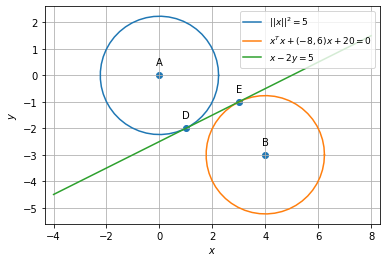
\includegraphics[width = \columnwidth]{a_3.png}
    \caption{Graphical illustration}
\end{figure}
\end{document}
